% This is part of Un soupçon de mathématique sans être agressif pour autant
% Copyright (c) 2015
%   Laurent Claessens
% See the file fdl-1.3.txt for copying conditions.

\begin{exercice}\label{exo2smath-0167}

    Le drapeau de la République Tchèque est comme ceci :
    \begin{center}
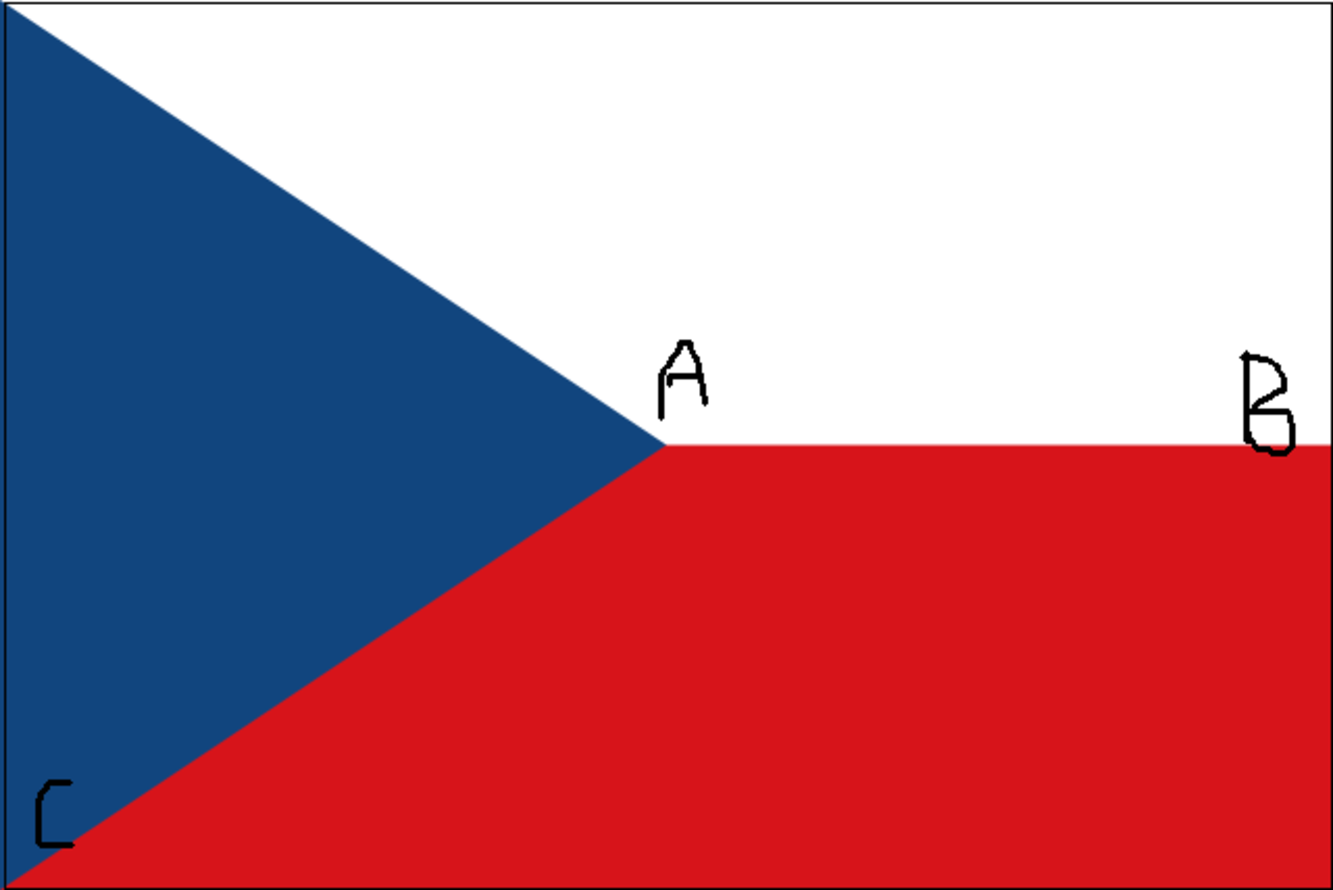
\includegraphics[width=5cm]{Czech_Republic.pdf}
    \end{center}
    Sachant que l'angle de la partie bleue en \( A\) mesure \SI{70}{\degree}, déterminer les deux autres angles de sommet \( A\).

    
\corrref{2smath-0167}
\end{exercice}
